\documentclass[problem]{mcs}

\begin{pcomments}
  \pcomment{PS_coin_flip_sequences}
  \pcomment{from: S09.ps11}
  \pcomment{subsumed by PS_prob_space_symmetry and CP_coin_flip_sequences}
\end{pcomments}

\pkeywords{
  conditional_probability
  total_probability
  transitive
  intransitive
  infinite_tree
}

%%%%%%%%%%%%%%%%%%%%%%%%%%%%%%%%%%%%%%%%%%%%%%%%%%%%%%%%%%%%%%%%%%%%%
% Problem starts here
%%%%%%%%%%%%%%%%%%%%%%%%%%%%%%%%%%%%%%%%%%%%%%%%%%%%%%%%%%%%%%%%%%%%%

\begin{problem}

\bparts

\ppart Suppose you repeatedly flip a fair coin until you see the sequence
\STR{HHT} or the sequence \STR{TTH}.  What is the probability you
will see \STR{HHT} first? 

\hint Use a bijection argument.

\begin{solution}
In this case the answer is $1/2$.  The proof is by a bijection
argument on the sample space.  Let $A$ denote the event that you see
\STR{HHT} before \STR{TTH}, and $B$ denote the event that you see
\STR{TTH} before \STR{HHT}.

We will define a bijection $g$ between $A$ and $B$ so that the
probability of $g(w)$ is equal to the probability of $w$.  The bijection
is quite simple.  Given a sample point $w \in A$, define $g(w) = \bar{w}$,
where $\bar{w}$ is the outcome where every \STR{H} is replaced by a
\STR{T} and vice versa.  For example $g(\mathtt{HHT}) =
\overline{\mathtt{HHT}} = \mathtt{TTH}$.

To show that $g$ is a bijection, we first observe that $g:A \rightarrow
B$.  This follows from the fact that \STR{HHT} precedes \STR{TTH} in
$w$ iff $\overline{\mathtt{HHT}} = \mathtt{TTH}$ precedes
$\overline{\mathtt{TTH}} = \mathtt{HHT}$ in $\bar{w}$.  And $g$ is onto by
the same reasoning.  Since $g$ is clearly an injection, we can conclude
that it is a bijection.

Then we observe that $\prob{w} = \prob{g(w)}$ for any $w$.  This is because
$\prob{\heads} = \prob{\tails}$ and $g(w)$ has the same length as
$w$.  Hence,
\[
\prob{A} = \sum_{w \in A} \prob{w} = \sum_{w\in A} \prob{g(w)}
= \sum_{w' \in B} \prob{w'}  =  \prob{B}.
\]
The second equality is valid because $g$ preserves the probability, and
the third by the bijection property with $w' = g(w)$.  Note that the fact
that \STR{H} and \STR{T} are equally likely is critical in these
calculations; this analysis would fail for a biased coin.

Finally we have to show that $\prob{A \union B} = 1$.  This follows from the
fact that the only way never to throw either pattern is to throw all
\STR{H}'s or all \STR{T}'s after the first toss, and we know that
the probability of there being an unbounded number of tosses of only H or
only T is zero.  That is, $\prob{\overline{A \union B}} = 0$ and so $\prob{A
\union B} = 1$.  Since $A$ and $B$ are disjoint, this means that $\prob{A} +
\prob{B} = 1$ and hence
\[
\prob{A} = \frac{1}{2}.
\]
\end{solution}

\ppart What is the probability you see the sequence \STR{HTT} before
you see the sequence \STR{HHT}?

\hint Try to find the probability that \STR{HHT} comes before
\STR{HTT} conditioning on whether you first toss an \STR{H} or a
\STR{T}. Somewhat surprisingly, the answer is not $1/2$.

\begin{solution}
\begin{solution}
We apply the standard tree diagram approach where the $n$th level of
the tree corresponds to the results of the $n$th coin flip.  This tree
is infinite, but we need not be intimidated: the tree has a repeating
structure which allows a simple recursive description.  Then the Law
of Total Probability applied to the recursive tree structure will lead
to some simple equations for the desired probability.

To see how this works, suppose our first toss is \STR{T}.  Since
neither of our patterns starts with \STR{T}, the situation relevant to
our patterns is the same as at the start.  So if we let $A$ be the
tree diagram describing our coin flipping experiment, then the branch
corresponding to flipping \STR{T} goes to a copy of $A$.  This is
illustrated in Figure~\ref{HTTHHT}.

\begin{figure}[h]
  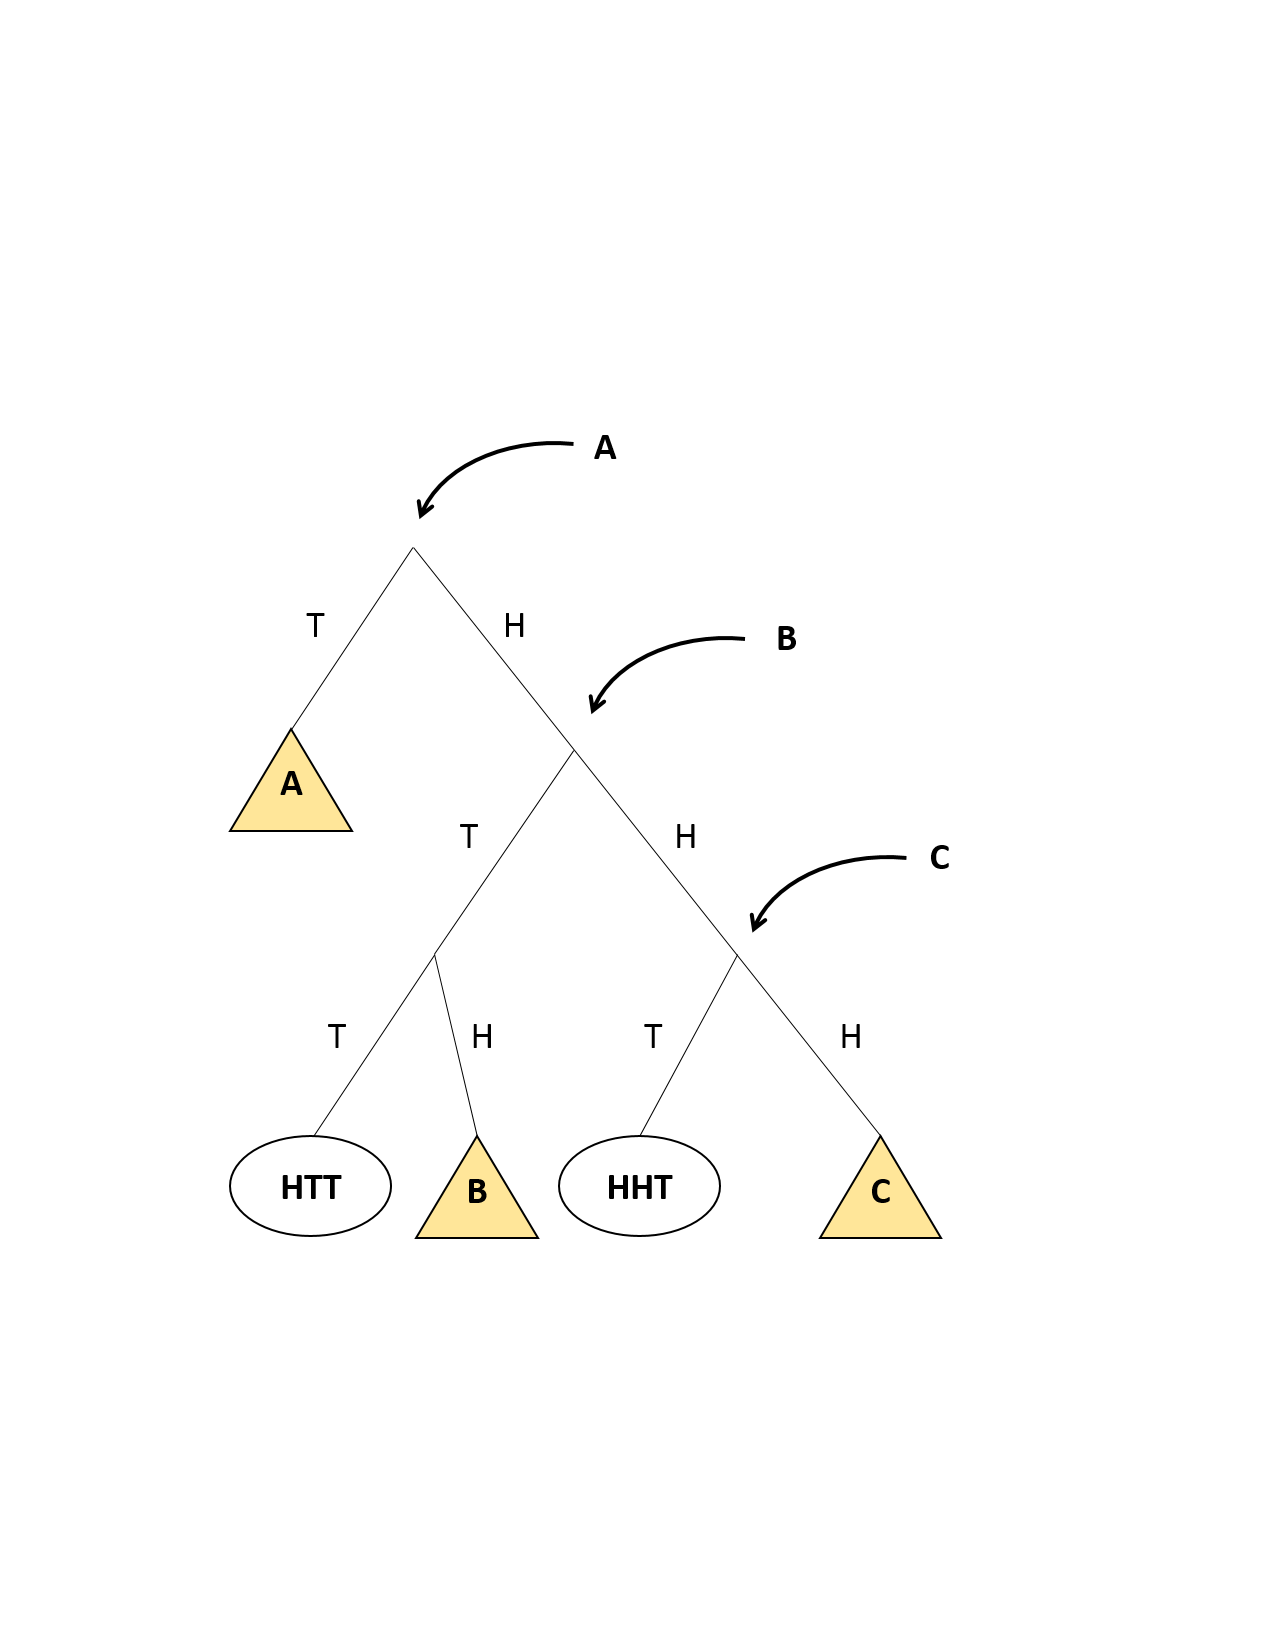
\includegraphics[width=4.5in]{HTT_HHT_race}
  \caption{\STR{HTT} versus \STR{HHT}.}
  \label{HTTHHT}
\end{figure}

If our first flip is \STR{H}, we need to consider different cases
based on the subsequent throws.  So let $B$ be the subtree
corresponding the first flipping \STR{H}, and let $C$ be the subtree
corresponding to the second flip also being \STR{H}.  Now if the third
flip is \STR{T}, then we arrive at the leaf where \STR{HHT} has
occurred first.  On the other hand, if the third flip is \STR{H}, then
the first flip is no longer relevant to the length three patterns we
are considering, and we are at the same point in progressing toward
our patterns as we were after flipping only two \STR{H}'s.  That is,
the \STR{H} branch of subtree $C$ is another copy of $C$.  This is
also illustrated in Figure~\ref{HTTHHT}.  We finish up by observing
that if the first three flips are \STR{HTT}, then we arrive at the
leaf where \STR{HTT} has occurred first, and if the first
three flips are \STR{HTH}, then the situation is the same as if we
first flipped \STR{H}.  So the subtree at after \STR{HTH} is the same
as $B$.

This completes the reasoning which led to the tree diagram illustrated
in Figure~\ref{HTTHHT}.

Now let $E$ be the event that \STR{HTT} appears before \STR{HHT}.  Our
task is to calculate $\pr{E}$.  Since the tree $A$ describes the start
of the coin flipping, we have
\[
\pr{E} = \prcond{E}{A}.
\]

Next, by the Law of Total Probability,
\begin{equation}\label{EAEAT}
\prcond{E}{A} = \prcond{E}{A} \cdot \pr{\STR{T}} + \prcond{E}{B} \cdot \pr{\STR{H}},
\end{equation}
which implies
\begin{equation}\label{EA=EB}
\prcond{E}{A} = \prcond{E}{B}.
\end{equation}

Again by the Law of Total Probability,
\begin{align}
\prcond{E}{B}
    & = \prcond{E}{B\STR{TT}} \cdot \pr{\STR{TT}}
       + \prcond{E}{B\STR{TH}} \cdot \pr{\STR{TH}}
       + \prcond{E}{B\STR{H}} \cdot \pr{\STR{H}}\notag\\
    & = 1 \cdot \frac14 + \prcond{E}{B}\cdot \frac14
            + \prcond{E}{C} \cdot  \frac12,\label{114EB}\\
\prcond{E}{C}
   & = \prcond{E}{C\STR{T}} \cdot \pr{\STR{T}}
       + \prcond{E}{C\STR{H}} \cdot \pr{\STR{H}}\notag\\
   & = 0 \cdot \frac12 +  \prcond{E}{C} \cdot \frac12. \label{012EC}
\end{align}
Now from~\eqref{012EC} we immediately get
\[
\prcond{E}{C} = 0.
\]
Then from~\eqref{114EB},
\begin{align*}
\prcond{E}{B} & = \frac14 + \prcond{E}{B} \cdot \frac14,\\
\prcond{E}{B} & = \frac13,
\end{align*}
and so by~\eqref{EA=EB}
\[
\prcond{E}{A} = \frac13.
\]
That is, \STR{HTT} appears before \STR{HHT} with probability 1/3.

These kind of events have an amazing \idx{intransitivity} property: if
you pick \emph{any} pattern of three flips such as \STR{HTT}, then I
can pick a pattern of three flips such as \STR{HHT} whose odds of
coming up first are better then even.  In particular, even if you
instead picked the ``better'' pattern \STR{HHT}, there is another
pattern I can pick that has a more than even chance of appearing
before \STR{HHT}.

\iffalse
So there are cases where a pattern 1 appears before a pattern 2 with
probability better than one half, and pattern 2 appears before a
pattern 3 with probability better than one half, and pattern 3 also
appears before pattern 1 with probability better than one half.
\fi

So we leave you with an ethical dilemma: is it OK to allow a naive
opponent to first choose whichever pattern of three flips he likes
best, then you choose your own preferred pattern, after which you bet
real money on the coin flip game?
\end{solution}

\eparts
\end{problem}

%%%%%%%%%%%%%%%%%%%%%%%%%%%%%%%%%%%%%%%%%%%%%%%%%%%%%%%%%%%%%%%%%%%%%
% Problem ends here
%%%%%%%%%%%%%%%%%%%%%%%%%%%%%%%%%%%%%%%%%%%%%%%%%%%%%%%%%%%%%%%%%%%%%

\endinput
